\documentclass{article}
\usepackage{ae,lmodern}
\usepackage[francais]{babel}
\usepackage[utf8]{inputenc}
\usepackage[T1]{fontenc}
\usepackage{graphicx}
\usepackage{float}
\begin{document}

\title{État de l'art : GeoLifeClef.\\Modèles d'apprentissage pour la prédiction d'espèces utilisant des variables environnementales. }
\author{Bourcier Jules, Karmim Yannis}
\maketitle


\clearpage
\section{Description de la tâche. }
Le but du challenge est de prédire une liste d'espèces sachant une localisation sur une carte de la France.
\\
\begin{figure}[h]
	\center
	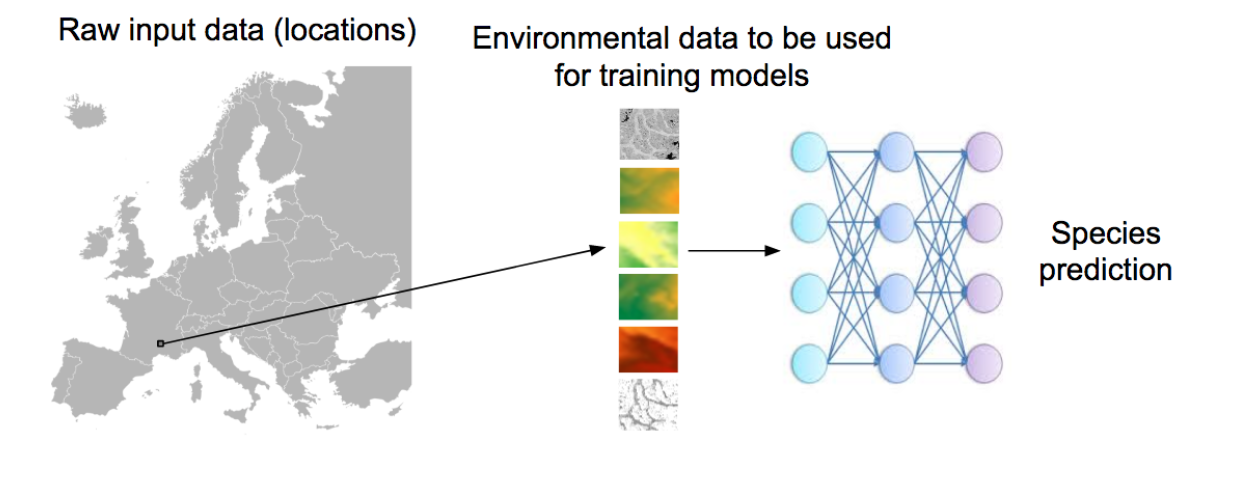
\includegraphics[width=10cm]{figure/figure1.png} 
	 \caption{Illustration de la tâche }
\end{figure}
\\
On possède une grande base de données d'espèces pour entraîner nos modèles, et chaque occurrence est accompagné d’un ensemble de 33 images de 64x64 pixels caractérisant l’environnement.
\\
Cependant il n'est pas possible d'apprendre la distribution des espèces directement des informations de localisation à cause du peu d'occurrences que l'on a pour certaines espèces et du biais d'échantillonnage car on a peu d’occurrences ou voir même pas du tout à certaines localisations)
\\
Ce qui est fait en écologie c'est de partir de la base d'une représentation d'un environnement. Typiquement un vecteur composé de la température moyenne de la  précipitation ainsi que d'autres variables comme le type de sol, la couverture terrestre, la distance à un point d'eau.\\
L'originalité de GeoLifeClef est d'utiliser des images pour représenter directement ces variables environnementales.
\\
Ces images sont un modèle en k dimensions, chaque patch représentant une valeur de variable de l'environnement ( température moyenne annuelle, max température du mois le plus chaud , précipitations annuel, l'altitude , la proximité à de l'eau fraîche ainsi que la capacité d'eau disponible.
\\
On se ramène à un problème de machine learning de "multi channel image classification task".
Chaque image représente une channel d'une variable d'environnement dans un carré centré dans la localisation.


\newpage
\subsection{Évaluation des modèles.}
Pour chaque occurrences du test les participants doivent classer par top 100 sans ex-aequo. \\L’évaluation métrique qu’on utilise s’appelle la MRR.
\begin{equation}
    \label{Formule pour calculer le score MRR.}
    MRR = \frac{1}{Q} \sum_{q=1}^{Q} \frac{1}{rank_{q}}
\end{equation}
Avec Q le nombre total d’occurrence $x_{q} $ dans l’ensemble de test et $rank_{q}$ est le rang correct de l’emplacement de l’espèce $y(x_{q})$ dans la liste des espèces évalué par la méthode pour l’occurrence $x_{q}$. \\La MMR est une mesure statistique permettant d’évaluer les processus qui renvoie une liste de valeurs possibles en réponse à une requête et ordonnés par la plus grande probabilité de vraisemblance.

\section{Étude des données.}
Chaque participants obtient des données d'apprentissages et de test des occurrences des espèces géo-localisées de variables ponctuelles d'environnement.\\ \\Les participants ont reçu une séries d'apprentissage et une série de test d'occurrences géolocalisées d'espèces. Les deux étaient d'abord composés d'un fichier.csv contenant les coordonnées spatiales des occurrences, les valeurs ponctuelles des variables environnementales à l'endroit de l'occurrence et, pour le tableau de l'apprentissage, le nom de l'espèce et son identificateur. Deuxièmement, chaque ligne du tableau (train et test) renvoie à une image à 33 canaux contenant le tenseur environnemental extrait à cet endroit.\\
Seules les données du territoires français ont été gardé car c’est un territoire bien connu et avec une biodiversité riche et variée.
Le label qu’on doit prédire dans le test sont dans le (field species GLC19SpId ). Toutes les espèces différentes sont associés à leurs noms scientifique qui sont donnés dans le champ scName.

\subsection{Données environnementales.}
Chaque occurrence pour un environnement est caractérisé par 33 images de $64*64$ pixels. Ces variables d’environnement ont été construite à partir de sources diverses. \\On a donc pour chaque occurrences des tenseurs de taille $64*64*33$ pixels.
\begin{figure}[H]
	\center
	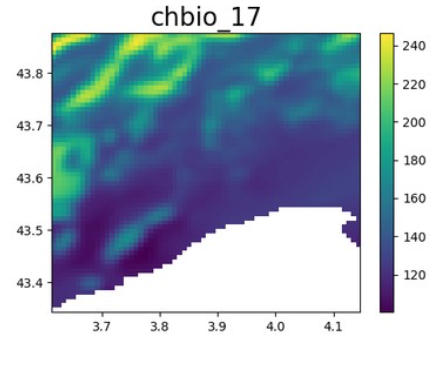
\includegraphics[width=7cm]{figure/figure2.png} 
	 \caption{chbio\_17 décrit le taux de précipitation de la période la plus sèche de l'année }
\end{figure}
\begin{figure}[H]
	\center
	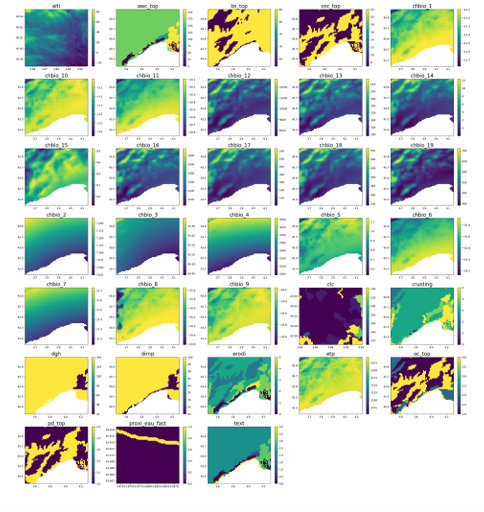
\includegraphics[width=7cm]{figure/figure3.png} 
	 \caption{Exemple de 33 images décrivant un environnement à une localisation précise.}
\end{figure}
\begin{figure}[H]
	\center
	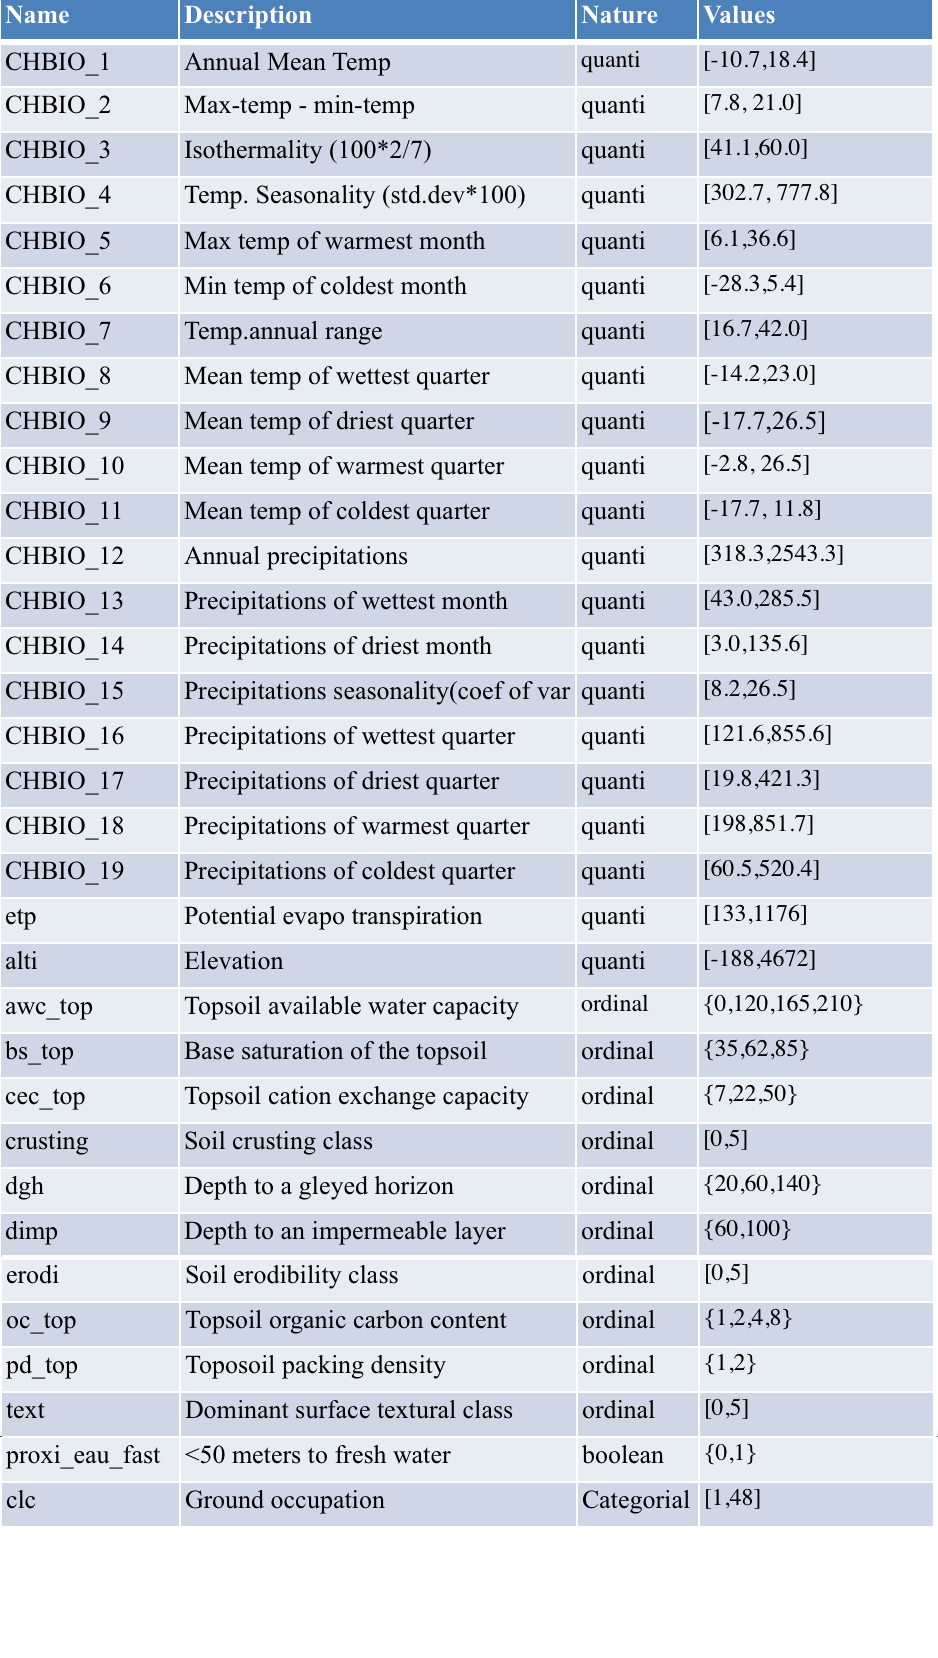
\includegraphics[width=9cm]{figure/figure4.png} 
	 \caption{Tableau descriptifs des 33 caractéristiques d'un environnement.}
\end{figure}
\subsection{Données et fichiers textes.}
\subsubsection{Ensemble de test.}
L’ensemble de test du challenge n’est pas fourni de base, il n’est publié qu’en mars. Pour chaque espèce présentes dans le test il y a au moins une observation dans l’apprentissage.\\ Une observation d’espèce dans le test est distante d’au moins 100 m des toutes observations de cette espèce dans l’ensemble d'entraînement pour éviter que ce soit trop facile à prédire.
\subsubsection{Ensembles de données d'occurrences.}\underline{Pl@ntNet complete dataset.}
\\
\\
Le fichier PL\_complete.csv contient 2 377 610 occurrences de 3 906 espèces. Dans le CSV, le champ \textit{FirstResPLv2Score} donne la confidence du score de prédiction automatique des espèces identifiées. Ce dataset est très hétérogène dans la qualité des identifications. Le champ accuracy donne l’incertitude en mètres calculée principalement par les smartphones.
\\
\\
\underline{Pl@ntNet trusted dataset.}
\\
\\
Le fichier PL\_trusted.csv où un filtre de confidence dans l’identification a été appliqué au Pl@ntNet complete dataset. Les occurrences gardées sont seulement celles ayant une probabilité d’identification pour la première espèce supérieure à 0.98. Ce score a été déterminé par des experts pour donner un degré raisonnable de vraisemblance dans l’identification. Cela a enlevé 90\% des occurrences. Cet un ensemble de 237 087 occurrences couvrant 1 364 espèces avec une géolocalisation et une identification précise n’a jamais été utilisé précédemment.
\\
Dates : début 2017 - novembre 2018.
\\
\\
\underline{GeoLifeClef 2018 dataset.}
\\
\\
Le fichier GLC\_2018.csv contient 281 952 occurrences couvrant 3 231 espèces. Avec ce dataset, les occurrences sont souvent agrégées au même point géographique, ce qui dénote des géolocalisations dégradées.\\ Le champ \textit{coordinateuncertaintyinmeters}, quand il est présent, informe sur l’incertitude de localisation.
\\
\\
\underline{NoPlant dataset.}
\\
\\
Le fichier noPlant.csv contient 5,771,510 occurrences couvrant 23,893 taxons. Aucune de ces espèces n'apparaîtra dans l’ensemble de test. Mais ce dataset complémentaire peut être utilisé pour améliorer la puissance prédictive des modèles en utilisant les corrélations fortes entre espèces de plantes et les autres taxons.

\section{Analyse des données par les participants de GLC 2018.}
Sur les 22 groupes ayant participé au challenge de 2018, seuls 3 ont rendu des résultats.\\ 
• Team ST \\
• Team FLO\\
• Team SSN \\
\subsection{Team : ST}
Les images ont été donné sous deux formats, un format image et un fichier .csv contenant les valeurs singulières.\\
La team ST a voulu extraire les valeurs singulières pour chacune des 33 images des occurrences, mais ils ont remarqué que certaines valeurs singulière étaient manquantes pour certaines images.\\Ils ont donc décidé de construire leurs propres valeurs singulières pour les images mais ils ont également vu que ce n’était pas possible de reproduire les mêmes que celles qui ont été donné.\\Ils ont recalculé les valeurs singulières pour toutes les images en faisant une moyenne des 4 pixels centraux.\\ 
En raison de ces différences ils concluent que c’est peut être à cause de cela qu’il y a une différence entre le test et l’apprentissage pour le calcul des valeurs singulières. \\
Ensuite ils ont comptés les valeurs singulières pour chaque classe et ont crée un diagramme par classe où sont  les plus probables pour chaque classe, les classes représentant les milieux environnementaux, et les ont comptés pour pouvoir avoir une identification pour chaque classe, identification qui sera la valeur singulière qui apparaît le plus dans la classe.\\
ST team suppose que les images des 33 channels n’ont pas tous la même influence sur la classification de l’environnement, ils ont donc essayé de déterminer quel sont les images avec le plus de “poids”. \\Pour chaque classe d’environnement ils ont créé une map de chaleur afin de déterminer ce qui caractérise une classe, cette map contient les valeurs moyennes de chaque images de cette classe.\\

\begin{figure}[H]
	\center
	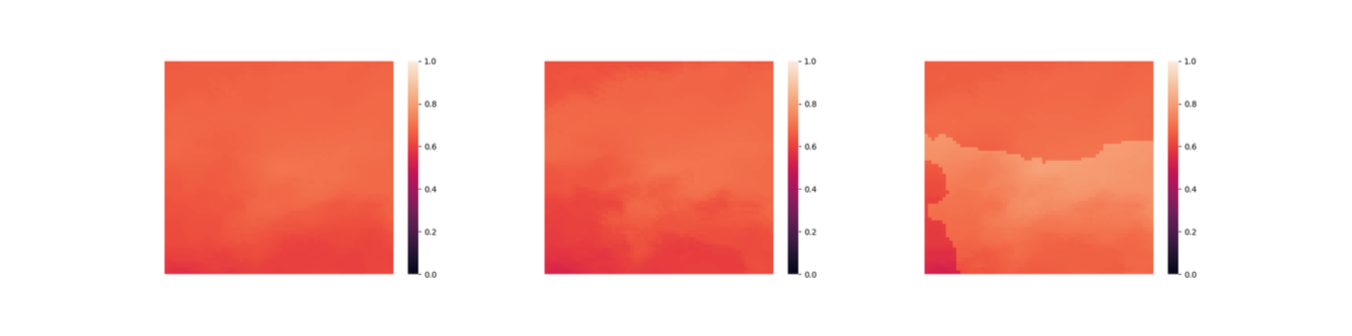
\includegraphics[width=9cm]{figure/figure5.png} 
	 \caption{Les maps de chaleurs des 3 classes les plus communes pour la classe 12 (précipitation annuelle).}
\end{figure}
L'équipe ST a utilisé 90\% des datas en apprentissage, le reste étant pour le test.
\subsection{Team : FLO}
L'équipe FLO spécifie uniquement qu'elle a utilisé 75\% des datas en apprentissage et le reste en test, mais n'a pas donné d'informations particulière sur les moyens qu'ils ont utilisés pour l'extraction et le pre-processing des données.\\


\subsection{Team : SSN}

Pour le challenge 2018 il y avait 3336 espèces différentes identifiées dans les données de test et d'apprentissage. L'équipe SSN a décidé de les regrouper par leurs caractéristiques communes en s'aidant de leurs noms taxinomiques. \\Ils ont supposés que des espèces similaires avaient plus de chance d'être géolocalisé au même endroit.\\ 
En effet la taxinomie fonctionne par hiérarchie, et en montant dans les hiérarchies on peut regrouper plusieurs espèces.\\

\begin{figure}[H]
	\center
	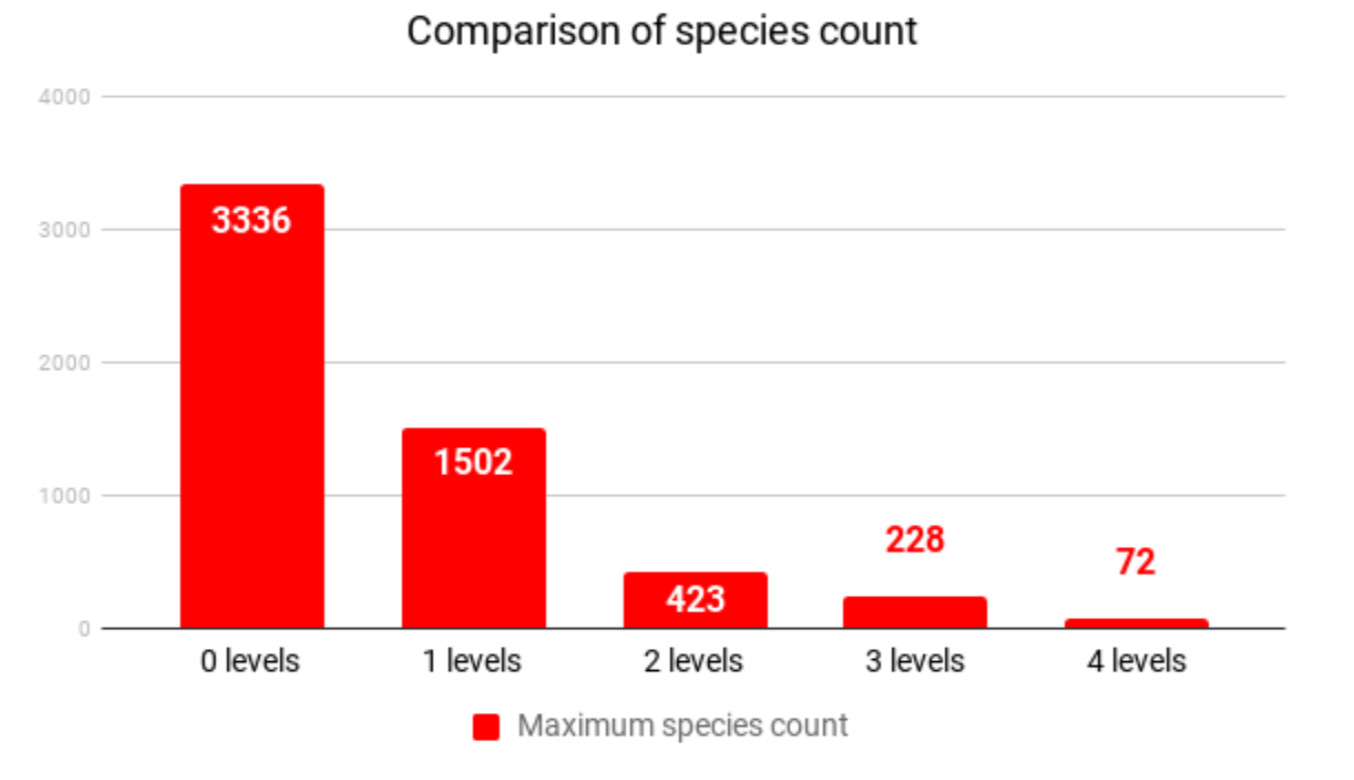
\includegraphics[width=9cm]{figure/figure6.png} 
	 \caption{Diagramme montrant le nombre de groupe d'espèces différents en utilisant $n$ hiérarchies taxinomiques. }
\end{figure}

\section{Les différents modèles de Machine Learning utilisés pour GLC 2018.}
Dans cette section on s'intéressera aux différents modèles de ML implémentés par les équipes du challenge 2018.\\
À noter qu'en plus des approches naïves il y a deux principales approches différentes pour entrainer les modèles. L'approche spatiale, qui grossièrement essaie d'apprendre en fonction des localisations où les espèces occurrent. Puis l'approche environnemental, qui elle apprend des variables d'environnements, c'est à dire des 33 images de taille $64*64$ caractérisant une localisation.\\ Nous allons détailler toutes les méthodes de ces approches qui ont été utilisées par les participants.

\subsection{Modèles naïf.}
\subsubsection{Modèles aléatoires.}
L'équipe ST a implémenté un modèle aléatoire pour donner une idée d'un mauvais score pour cette tâche.\\Ils ont choisi pour le top 100 aléatoirement dans les 3336 espèces différentes et ont retourné cette liste.\\ L'execution correspond à [ST\_2] et a eu un score de 0.0016.

\subsubsection{Modèle probabiliste.}
L'équipe ST a utilisé  un modèle purement probabiliste. Ce modèle comptait toutes les espèces dans l'ensemble des données d'apprentissage, et en les triant par plus haute fréquence.\\Pour le test l'algorithme retournait toujours le même top-100 des espèces qui apparaissaient le plus.\\L'execution correspondait à [ST\_7] et a obtenu un score de 0.0134.

\subsection{Modèle vectoriel.}
L'équipe ST a développé un modèle vectoriel simple. \\
Ce modèle a pour objectif de calculer la différence entre les occurrences de l'apprentissage et du test.
Ils ont construit pour chaque occurence un vecteur $V$ à 33 dimensions, la dimension $k$ étant la valeur moyenne des 4 pixels centré sur l’occurence de la variable d’environnement k.\\
Le modèle calcul la distance de cette façon :\\ \\
$\overrightarrow{V}_{n} = $ $n$ -ième vecteur de l'occurrence d'apprentissage \\
$\overrightarrow{V}_{m} = $ $m$ -ième vecteur de l'occurrence de test \\
$\overrightarrow{V}_{nm} = \overrightarrow{V}_{n} - \overrightarrow{V}_{m} $\\
$ D_{nm} = || \overrightarrow{V}_{nm} ||_{2}$\\
À chaque occurence de l’ensemble d’apprentissage. Les distances $D$ sont triés par ordre croissant de distance. Les 100 plus proches classes distinctes sont retournées, en ne conservant que la plus proche occurence d’une espèce quand celle-ci apparaît plusieurs fois.\\
Ce modèle peut s'apparenter à un k plus proches voisins.
Le MRR de ce modèle est 0.0271.




\subsection{Boosted Trees.}
L'équipe ST a développé une approche en se basant sur l'usage de XGBoost (Extreme Gradient Boosting). \\
Avec cette méthode il affirme qu'il est possible de prédire une variable cible basé sur les caractéristiques des données d'apprentissage.\\
Pour rappel le boosting est une technique utilisée en apprentissage statistique qui a pour but de combiner des classifieurs simple séquentiellement, à quoi on attribue un certain poids, afin d'optimiser les performances de prédiction.\\ Le gradient boosting a pour particularité d'utiliser le gradient de la fonction de perte pour calculer les poids des classifieurs. Les classifieurs ici sont généralement des arbres binaires de décision (CART) de profondeur pas trop grande pour éviter le sur-apprentissage.\\ Il y a un unique paramètre à choisir, qui est la profondeur de l'arbre $max\_depth$.\\
Ils ont eu plusieurs stratégies pour l'implémentation des Boosted Trees. 
\subsubsection{Modèle unique.}
La première stratégie a été de faire un modèle unique pour la prédiction, dans ce cas la variable cible est une liste des probabilités des espèces pour chaque occurrence des données de test.\\
L'équipe a soumis 3 executions en faisant varié la profondeur de l'arbre et en utilisant l'évaluation MRR.\\
$max\_depth = 10 $  :  $ Test-score = 0.0085 $\\
$max\_depth = 3 $    :  $ Test-score = 0.0344 $\\
$max\_depth = 2 $    :  $ Test-score = 0.0348 $\\
Comme il est dit précédemment, une faible profondeur de l'arbre évite le sur-apprentissage.
\subsubsection{Multi-modèles.}
La seconde stratégie a été de prédire chaque espèce séparément, comme il y avait 3336 espèces, ils ont créé 3336 différents modèles.\\
In this case the target variable mentioned earlier was a list of probabilities for the occurrence of the current selected single species (one out of 3336) for a dataset occurrence. Each model was evaluated during the training with the log-loss metric because the resulting probabilities were decimal numbers.\\
\subsubsection{Modèle de groupe.}
Ensuite la dernière méthode a été d'utiliser des modèles de groupes.\\
Il est probable que plus d’une espèce apparaissent à un même endroit. Partant de cette idée, ST a proposé un modèle utilisant un groupement d’espèces similaires.\\Pour trouver des similarités, on calcule pour chaque espèce, un vecteur représentatif : à partir des les occurrences de l’espèce dans l’ensemble d’apprentissage, ils ont calculé les valeurs moyennes des 33 variables (sur les 64x64 pixels).\\
Ensuite ils on calculé la distance entre ces vecteurs (comme pour le modèle vectoriel) ce qui donne une matrice de taille $3336x3336$ dans laquelle la distance entre chaque espèce est stockée. En ignorant les espèces qui ont moins de $o$ occurrences.\\
Le paramètre $t$ est un seuil indiquant la distance maximum pour que deux espèces appartiennent au même groupe.\\
Cela n’est pas suffisant pour apporter de la similarité :\\\\
\begin{figure}[H]
	\center
	\includegraphics[width=9cm]{figure/figure8.png} 
	 \caption{Chaque point représente une espèce et les arêtes sont les distances entre les espèces à une distance maximale $t$.Le problème est que parfois entre des espèces du même groupe il peut y avoir une distance de $3t$ ce qui n'est plus très proche. }
\end{figure}
Ils ont donc introduit un paramètre $min\_edges$ qui donne le nombre de voisins dans un rayon de taille maximal $t$. Cela donne moins de groupe mais il y a une meilleure similarité.\\
\begin{figure}[H]
	\center
	\includegraphics[width=9cm]{figure/figure7.png} 
	 \caption{Maintenant il y a une meilleure similarité en utilisant le paramètre $min\_edges = 3 $. }
\end{figure}
Enfin pour une occurrence de test, on calcule le groupe de cette occurrence. Puis pour retrouver l’espèce, on retourne les espèces de ce groupes par fréquences décroissantes dans l’ensemble d’apprentissage.\\Pour les paramètres $min\_edges = 3$, $t = 9 $ et $o = 0$, ce modèle a obtenue une MRR de 0.0326.

\end{document}












